\chapter{实验结果与分析}
本章节主要是对此前在UPMEM上进行软硬优化的GEMV算子的综合测试,第一小节介绍环境配置平台,第二小节重点测试UPMEM近存计算硬件平台的GEMV算子总计算能力,并与其他常见的硬件计算平台进行对比,第三小节重点测试在UPMEM上的GEMV算子优化的效果和运行时间的细分(breakdown),分析瓶颈和优化空间;第四小节介绍GEMV算子的扩展性,分析改算子在矩阵尺寸发生变化时的通用性。

\section{环境配置介绍}

\subsection{硬件平台}
我们实验的近存计算平台是在UPMEM官方建议的UPMEM服务器上,该服务器配备了双插槽的英特尔至强4210 CPU,每颗CPU拥有10个核心20个线程,每个核心工作在2.20GHz的基准频率,拥有32KB的L1缓存、1MB的L2缓存和13.75MB的L3缓存。每个CPU配备6个内存通道,支持DDR4-2400的内存。我们为每个CPU的5个通道插满UPMEM DIMM,剩余的一个通道配置常规DDR4-2400的内存。每个内存通道插入两根UPMEM DIMM,每个UPMEM DIMM上配有128个DPU。因此一共有$2\times 5\times 2\times 128=2560$个DPU可以同时工作,每个DPU的存储容量为64MB,因此UPMEM内存的存储容量一共是160GB。普通CPU内存有128GB。

同时实验对比使用的CPU平台是在配备了双插槽的英特尔至强6242 CPU的服务器平台上,每颗CPU拥有16个核心32个线程,每个核心工作在2.80GHz的基准频率,拥有32KB的L1缓存、1MB的L2缓存和22MB的L3缓存。每个CPU配备6个内存通道,支持DDR4-2933的内存。该平台上没有插UPMEM DIMM,全部配备的是标准DDR4内存共256GB。之所以CPU平台和UPMEM平台要分开成两套硬件测试,而不能复用UPMEM平台的原因是,UPMEM平台的CPU的6个内存通道有5个都被UPMEM占用,CPU内存传输带宽变为原来的六分之一,这样的对比实验并不公正。

GPU的硬件装配在CPU平台上,由于通过PCIE接口连接而并不影响性能。GPU平台配备了一块Nvidia A6000 GPU,其核心代号为GA102,安培架构,拥有10752个CUDA Core和336个Tensor Core,单精度浮点性能达38.7TFLOPS。其拥有48GB的GDDR6显存,384bit的传输位宽,显存带宽能达到768GB/s,足以容纳我们评估中使用的数据。

% 具体详细的硬件配置可以见\ref{table:experimental-setup}
% \begin{table}[h]
%     \caption{TABLE I: Experimental Setup}
%     \begin{tabular}{|l|l|l|}
%     \hline
%     & \multicolumn{2}{|c|}{} \
%     \cline{2-3}
%     \multirow{-2}{}{PIM Platform} & HOST & \begin{tabular}{l}
%     Xeon 4210 CPU  2 \
%     128G DDR4 Memory
%     \end{tabular} \
%     \hline
%     & DRAM - PIM & \begin{tabular}{l}
%     UPMEM PIM - DIMM  20 \
%     2560 PEs, 160G DDR4 Memory
%     \end{tabular} \
%     \hline
%     \multirow{2}{}{GPU Platform} & HOST & \begin{tabular}{l}
%     Xeon 6242 CPU  2 \
%     256G DDR4 Memory
%     \end{tabular} \
%     \cline{2-3}
%     & GPU & Nvidia A6000 \
%     \hline
%     \end{tabular}
%     \label{table:experimental-setup}
% \end{table}

\subsection{数据准备和矩阵尺寸选择}
我们选择被广泛使用的开源模型Llama2-7b-chat,使用WikiText2\footnote{https://huggingface.co/datasets/mindchain/wikitext2/tree/main}和PTB\footnote{https://aistudio.baidu.com/datasetdetail/67}作为量化校准数据集对原始权重进行FP8/FP4量化,以机器学习的方式构建FP8/FP4查找表,以随机选取的量化后的权重矩阵(MHSA中的线性层)作为测试数据。我们在主要的算子吞吐测试和优化细分测试中选择两种不同的GEMV数据尺寸,分别是$4096\times 256$,$256\times 4096$,分别对应Llama2-7B推理过程中可能出现的窄的降维矩阵和宽的升维矩阵(选择256维度方便与SIMD指令的测试统一维度),在扩展性测试中我们将使用不同矩阵尺寸进行测试。在数据宽度方面,近存计算平台分别选择Float32和FP8(E4M3)两种数据格式进行测试,相应的在CPU和GPU平台选择Float32和INT8进行测试(硬件不支持FP8)。每个DPU使用$4096\times 256$尺寸的矩阵,用满UPMEM所有DPU进行总的吞吐测试,矩阵的大小为$4096\times 256\times 2560$,假设采用32bit的数据格式,矩阵所占空间最大为$4096\times 256\times 2560\times 4=10GB$,上述硬件平台足以存储。

\subsection{基线设置}
对于PIM平台,真实硬件的测评使用UPMEM SDK(版本 2024.1.0)编译在UPMEM-DIMM执行,模拟器的优化工作通过比较真实硬件性能和周期推算性能表现。我们在近存计算硬件UPMEME上的优化分别与CPU和GPU平台的Float32和INT8推理做比较,CPU平台使用英特尔数学核心函数库(Intel Math Kernel Library,MKL)\cite{IntelMKL},是英特尔官方开发的一套高性能数学计算库,里面包含BLAS接口,针对Intel(至强处理器)硬件特性进行了深度优化(如使用SIMD指令和寄存器),同时能够简单高效地支持多线程和并行计算。而GPU平台我们将基于CUDA(12.2)使用cuBLAS库\footnote{https://docs.nvidia.com/cuda/cublas/index.html}:cuBLAS是NVIDIA官方开发的一个高性能线性代数库,专为CUDA平台设计,充分利用了NVIDIA GPU的硬件特性,能够显著加速矩阵乘法(GEMM)、向量运算和其他线性代数任务。对于下发的任务包括GEMV,在支持Tensor Core的GPU硬件上,cuBLAS会自动优化选择使用Cuda Core还是Tensor Core以到达最佳性能。

\section{GEMV算子运算性能和能效比对比}

\subsection{GEMV算子运算性能对比/}
GEMV算子的运算性能我们选择性能指标每秒浮点运算次数(Floating-point Operations Per Second, FLOPS)来衡量,对于矩阵尺寸为$M\times N$的GEMV操作来说,具体的计算公式为\ref{GFLOPsEqu},其中Latency为GEMV算子的时延,单位为秒。\ref{EXP1-1}分别显示了在近存计算平台(UPMEM)、CPU平台和GPU平台上的GEMV算子运算性能,UPMEM使用了全部2560个DPU,每个DPU配置16个tasklet。

\begin{equation}
    GFLOPs=\frac{2\times M\times N}{Latency}\times 10^9
    \label{GFLOPsEqu}
\end{equation}

\begin{figure}[!htbp]
    \centering
    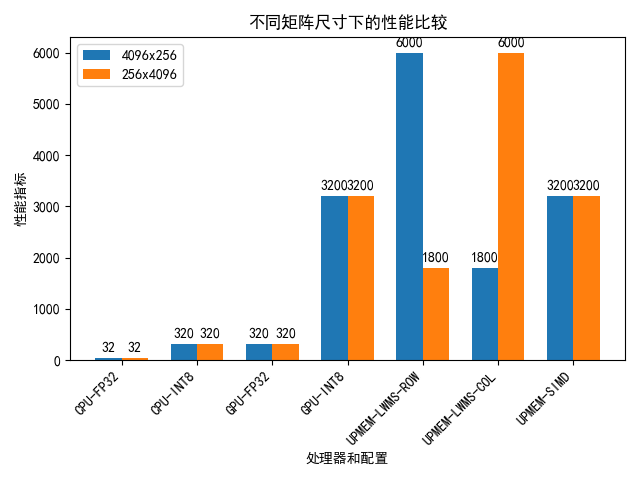
\includegraphics[width=0.9\textwidth]{figures/Exp1-1.png}
    \caption{}
	\label{EXP1-1} %% label for entire figure 
\end{figure}

可以看到无论是对于哪种矩阵尺寸,在UPMEM硬件平台上,GEMV算子的计算性能峰值能达387GFLOPS,远超CPU和GPU平台的计算性能。CPU平台的计算性能最差,原因大概是因为10GB的矩阵数据量庞大,CPU花费大量时间参与矩阵数据的搬移工作,表现为严重的内存瓶颈。GPU平台的计算性能表现良好,得益于GPU大量高度并行的CUDA计算核心和高速的内存带宽传输数据,但是在实验过程中我们通过Nsight工具观察到GPU的硬件利用率普遍不高。UPMEM经过精心调优的GEMV算子的计算性能最强,而且可以明显地看到对于窄的矩阵,行重排的优化效果最为明显,大概相比较CPU有12倍的提升,相较GPU有2倍的提升,而对于宽的矩阵,列重排的效果最为明显,相较于CPU有10倍的提升,GPU有1.5倍的提升。同时可以看到使用的SIMD指令的GEMV性能远高于其他算子,相较于CPU有15倍的提升,相较于GPU有3倍的提升,这得益于对于硬件的定制化修改以及更低位宽的权重量化。

\subsection{GEMV算子能效比对比}
近存平台的一大优势在于其减少了数据移动的开销从而能够更加节能,非常适合边端对功耗有严格要求的设备,因此我们在测试计算能力的同时也测试了各个硬件平台的能效比。我们使用Intel VTune Profiler来测试CPU平台上的能耗,同时使用Nsight工具来测试GPU平台的能耗。对于UPMEM平台,由于官方没有提供能耗测试工具,因此我们只能通过UPMEM SDK的dpu-diag工具测试DPU的内核和DRAM Bank的静态功耗,大约为12.8w每根DIMM条。能效比定义简单地计算公式为:\(EnergyEffiency=\frac{GFLPOPS}{Energy}\),其中GFLOPS为计算性能与上一小节中的测试结果保持一致,Energy为能耗,单位为GFLOPS/W。

\begin{figure}[htbp]
    \centering
    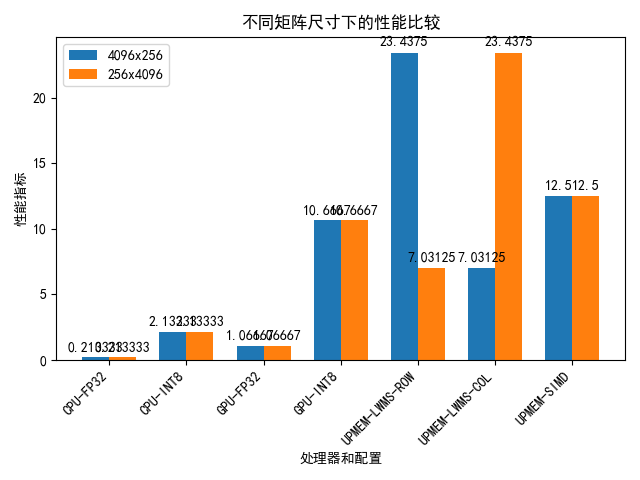
\includegraphics[width=0.9\textwidth]{figures/Exp1-2.png}
	\label{EXP1-2} %% label for entire figure 
\end{figure}

测试结果如\ref{EXP1-2}所示,CPU平台的能效比最差,其原因主要是由于CPU将大量的计算用于搬移数据而非计算,导致计算性能远低于其他两个硬件平台。GPU的能效比较为良好,得益于其本身强悍的内存带宽以及强大的计算性能。UPMEM的能效比在三者之间最高,平均达到了CPU的5倍,GPU的1.4倍,这主要是得益于所有DPU的超高的聚合带宽以及优化良好的软硬件协同设计。

\section{GEMV算子优化和执行时间细分}
\subsection{GEMV算子优化细分}
我们在第三章和第四章分析UPMEM的硬件特点,通过软硬协同设计一步一步优化了GEMV算子,为分析每步优化的有效性和对总体性能的影响,我们需要将每步优化拆来进行测试,具体测试结果如\ref{GEMVOpt}所示,所有的测试都在单DPU上进行,测试算子在特定矩阵尺寸下的执行时间,Tasklet数量设置为16。

\begin{figure}[htbp]
	\centering
	\subfigure[W8A8数据格式]{ 
		\label{GEMVOpt:W8A8} %% label for first subfigure 
		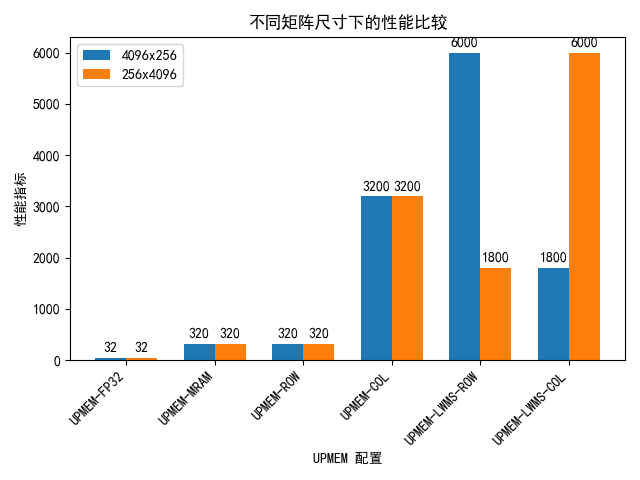
\includegraphics[width=0.45\textwidth]{figures/Exp2-1-1.png}
	}
	\subfigure[W4A8数据格式]{
		\label{GEMVOpt:W4A8} %% label for second subfigure 
		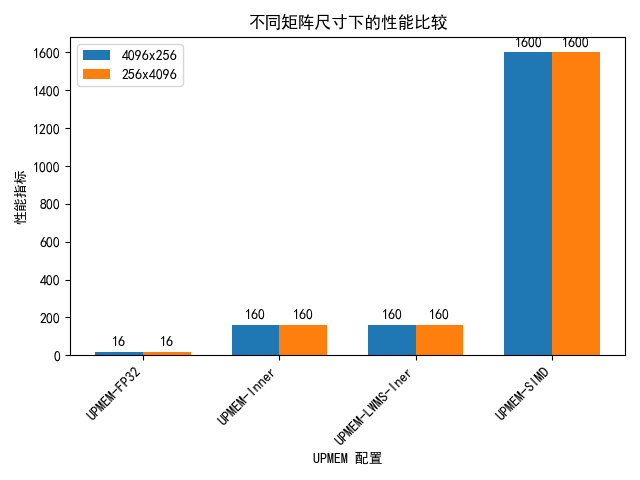
\includegraphics[width=0.45\textwidth]{figures/Exp2-1-2.png}
	}
    \label{GEMVOpt} %% label for entire figure 
	\caption{GEMV算子优化Breakdown}
\end{figure}

我们先看W8A8数据格式的优化\ref{GEMVOpt:W8A8},基准是未经优化的FP32的GEMV算子(UPMEM-FP32),然后是基于查找表分块的优化(UPMEM-MRAM),然后分别是在真实硬件上的行、列重排(UPMEM-ROW,UPMEM-COL)和模拟器上的基于新增FMA指令的行列重排优化(UPMEM-FMA-ROW,UPMEM-FMA-COL)。数据结果显示相较于UPMEM-FP32,UPMEM-MRAM的优化提升巨大,有30倍的提升;对于窄矩阵($4096\times 256$),行重排的提升有8倍,对于宽矩阵来说($256\times 4096$),列重排的提升大概2.5倍,但是行重排之于宽矩阵,列重排之于窄矩阵提升就不大了;在模拟器行增加了查找表专用的FMA指令后,平均提升大概3-4倍,与理论分析一致。

对于W4A8数据格式的GEMV算子优化,基准仍然是UPMEM-FP32,由于查找表可以完全放入WRAM因此没有多余的设计,在UPMEM上就是很简单地使用GEMV的内积效率就很高,因此第二个优化就是UPMEM-Inner,对于FP32的提升非常高达50倍;在模拟器上仍然可以使用FMA指令加速,提升大概也是3-4倍,使用SIMD指令加速提升大概有16倍,可以看到初开SIMD对权重数据位宽的要求外,SIMD指令用于查表的提升仍然很大。

\subsection{GEMV算子执行时间细分}
为了分析每种优化的的瓶颈,我们需要对每种优化下GEMV算子的执行时间进行细分,分别统计在计算(Arithmetic),访存(WRAM Load/Store),线程间同步(Synchronization),MRAM的数据传输耗时(DMA to/from MRAM),以及其他这6种操作上的耗时,分析瓶颈所在和优化有效性。我们仍然在单个DPU内测试,设置Tasklet的数量为16.

\begin{figure}[htbp]
	\centering
	\subfigure[W8A8-4096x256]{ 
		\label{GEMVTime:W8A8-4096x256} %% label for first subfigure 
		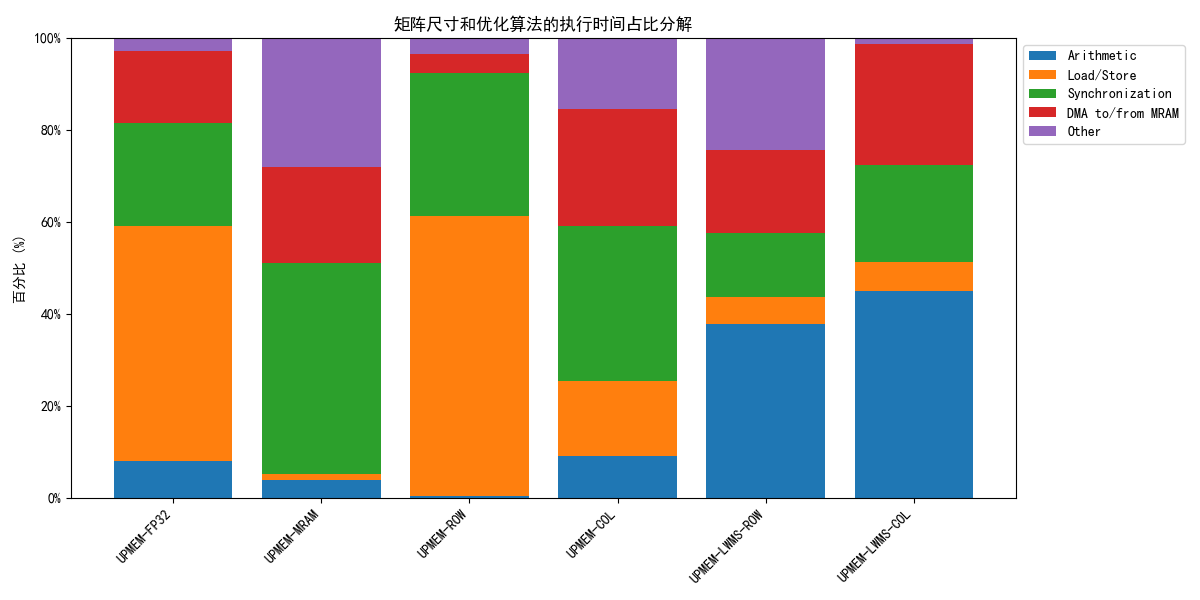
\includegraphics[width=0.45\textwidth]{figures/Exp2-2-1-4096x256.png}
	}
	\subfigure[W8A8-256x4096]{
		\label{GEMVTime:W8A8-256x4096} %% label for second subfigure 
		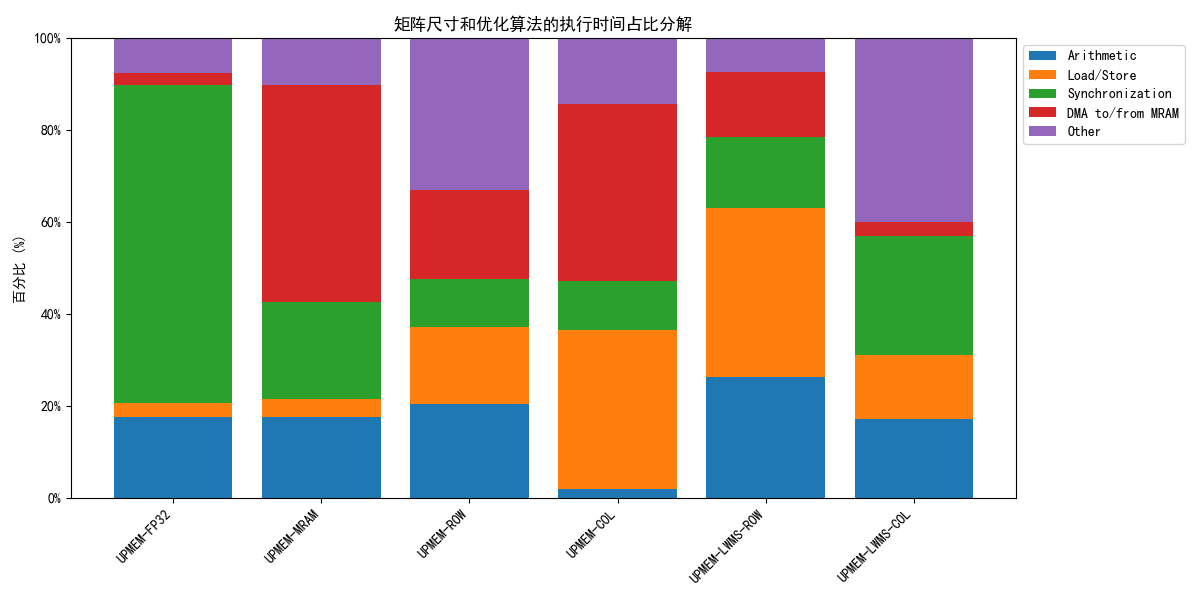
\includegraphics[width=0.45\textwidth]{figures/Exp2-2-1-256x4096.png}
	}
    \\
    \subfigure[W4A8-4096x256]{ 
		\label{GEMVTime:W4A8-4096x256} %% label for first subfigure 
		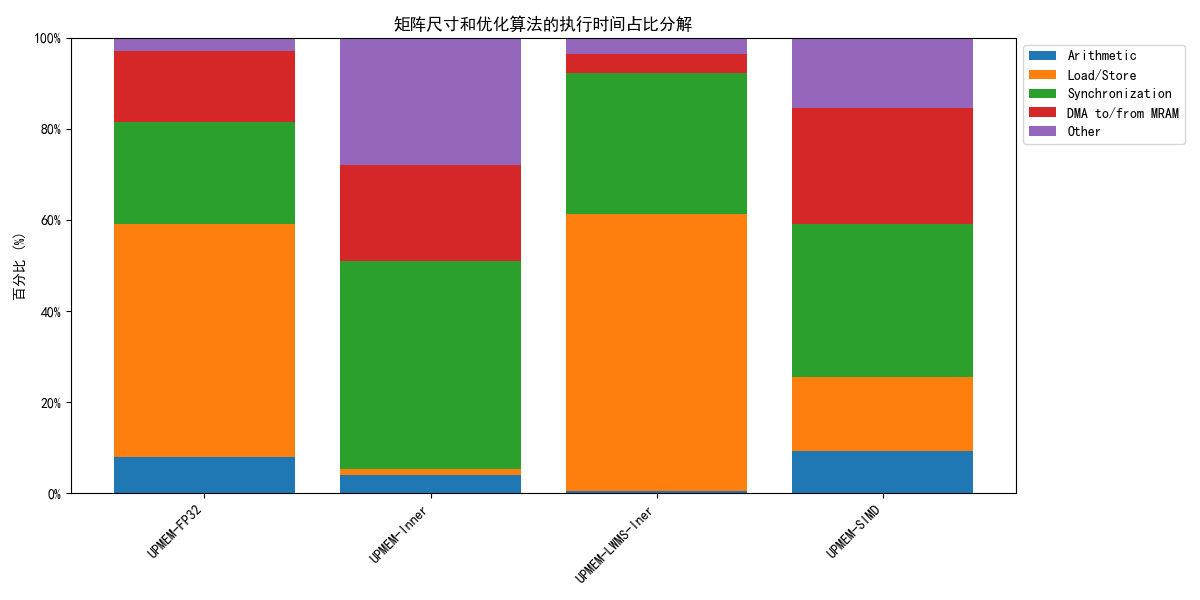
\includegraphics[width=0.45\textwidth]{figures/Exp2-2-2-4096x256.png}
	}
	\subfigure[W4A8-256x4096]{
		\label{GEMVTime:W4A8-256x4096} %% label for second subfigure 
		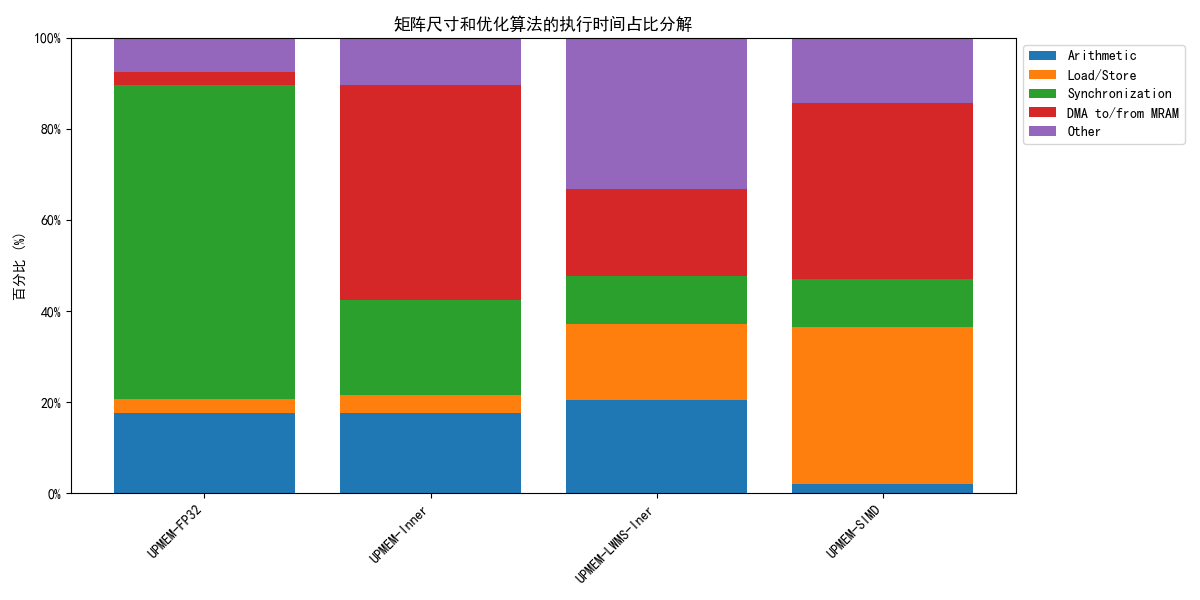
\includegraphics[width=0.45\textwidth]{figures/Exp2-2-2-256x4096.png}
	}
    \label{GEMVTime} %% label for entire figure 
	\caption{GEMV算子优化Breakdown}
\end{figure}

我们可以看到,UPMEM的绝大部份的时间都耗费在访存和计算上,同步时间和DMA时间都可以忽略不计,这说明我们的优化算法对于数据局部性的优化非常的成功同时高度利用了多线程并行化计算。

\section{扩展性测试}
扩展性测试可以分为强弱扩展性测试,所谓强扩展性就是在问题规模一定的情况下提高计算能力,而弱扩展性就是在问题规模变大时,等比例扩大计算能力使得总问题规模比上计算能力保持不变。在这里问题规模其实就是矩阵的大小,计算能力在大的粒度上可以认为是DPU的数量,在小的粒度上可以认为Tasklet的数量。由于GEMV可以按照列随意切分矩阵的粒度,因此在这里我们不考虑DPU粒度的计算能力,将具体实验测试限制在单个DPU中,同时由于Tasklet的特殊,我们取消弱扩展性测试改为负载能力测试,即给定计算能力下扩大数据规模,观察负载能力随数据规模的变化。

\subsection{强扩展性测试}
对于强扩展性测试,我们测试的矩阵大小分别是$4096\times 256$和$256\times 4096$,分别对应宽和窄矩阵,具体的GEMV算子我们选择W8A8数据格式下的行、列重排,即UPMEM-ROW-FMA,UPMEM-COL-FMA,W4A8数据格式下选择UPMEM-SIMD,设置Tasklet数量从1逐渐增加到24,测试各个算子的执行时间:

\begin{figure}[htbp]
    \centering
    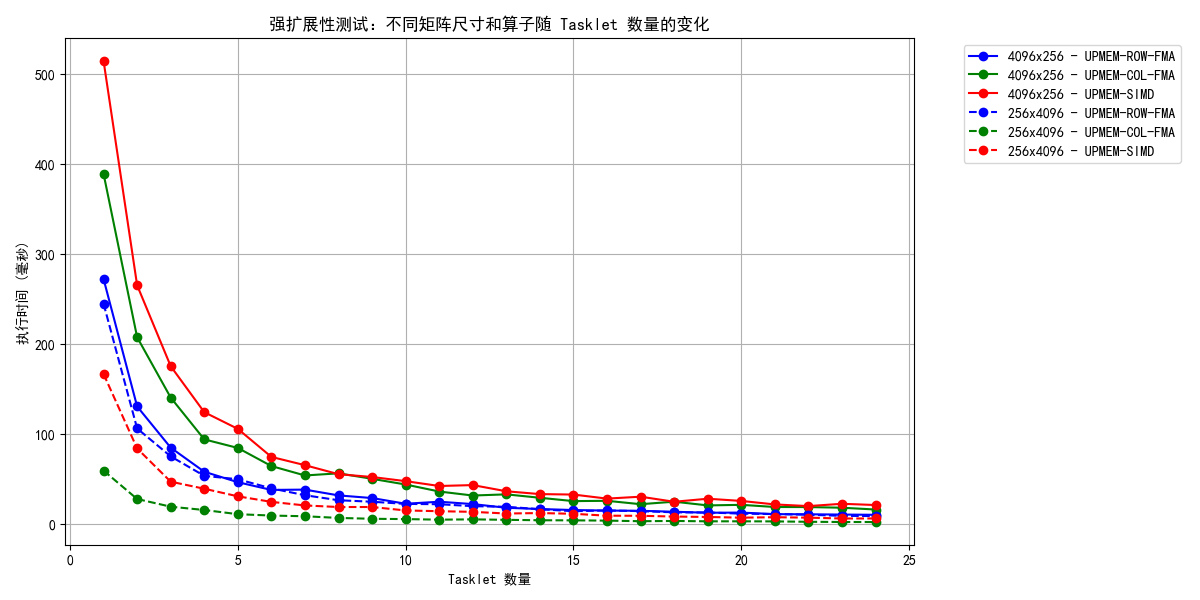
\includegraphics[width=0.9\textwidth]{figures/Exp3-1.png}
    \caption{}
	\label{EXP3-1} %% label for entire figure 
\end{figure}

可以看到随着Tasklet的增加各个算子的执行时间随之减少,当Tasklet超过11个时,计算达到饱和。

\subsection{负载能力测试}
我们同样选择UPMEM-ROW-FMA,UPMEM-COL-FMA,和UPMEM-SIMD这三个算子,设置Tasklet数量为16,改变工作负载,将矩阵的尺寸从$4096\times 256$翻倍变化到$4096\times 4096$,同样将$256\times 4096$翻倍变化到$4096\times 4096$,测试各个算子的执行时间:

\begin{figure}[htbp]
    \centering
    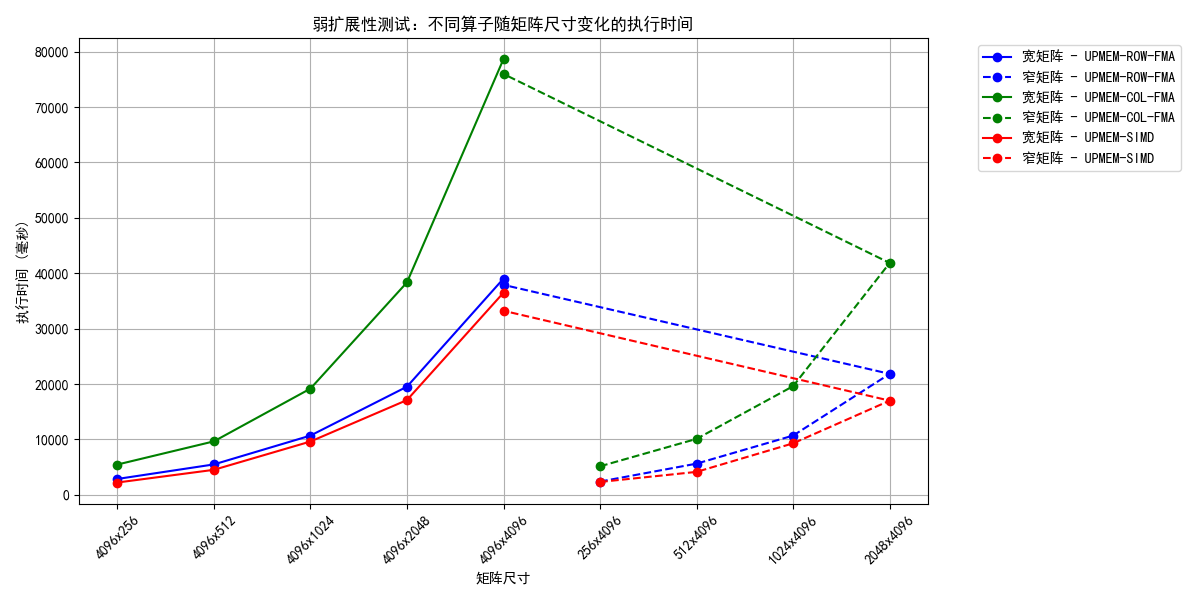
\includegraphics[width=0.9\textwidth]{figures/Exp3-2.png}
	\label{EXP3-2} %% label for entire figure 
\end{figure}
